\chapter{Location-Based Freecycling Service Prototype}
\label{cha:prototype}


\section{Introduction and Objective }
\label{sec:prototype_introduction}

The second phase of the study was the implementation of a location-based freecycling service prototype called ``Geofreebie''. The goal of this phase was to develop practical design solutions for a subset of the usage requirements developed in phase one. A secondary goal was to produce a usable prototype that would enable evaluation of the theories developed during the needs assessment.

This chapter discusses the details of the implementation and the rationale behind the design solutions. First we explain the technologies that were used and the rationale for choosing these technologies. Next, we provide an outline of the overall architecture of the system, including the configuration of the various services that make up the application and the interfaces that join them. After that we describe the structure and design of the back-end server and the architecture of the front-end user-facing mobile application. An overview of some key features of the mobile application and the considerations that contributed to their selection and development is discussed later in chapter~\ref{cha:discussion}.


\section{Technologies}
\label{sec:technologies}

We chose to implement the service as a mobile app because forced migrants are more likely to use smartphones than other hardware \cite{xu_communication_2016}. All of our interviewees had smartphones and cited them as their main means of communicating and one of their main tools when making new social contacts. Because most people carry their phones with them throughout the day, mobile apps also open up possibilities for spontaneous social contact in the moment and the location where the context is most apt.

We used the open source LBS-Engine, an application template for the development of location-based services, as a foundation for our app \cite{einfeldt_lbs_2018}. This sped up development by providing an initial framework for displaying a map, navigating via a tab bar and a sidebar, and presenting the user with various settings.

The LBS-Engine uses the open source Cordova framework from Apache, which allows mobile apps to be developed using web app technologies like JavaScript, HTML, and CSS. A major benefit of using Cordova is that once the application is developed, it can be easily ported to several different operating systems without rewriting the code. Currently supported operating systems include Android, iOS, OS X and Windows. This makes services developed with Cordova more accessible because they do not depend on the user having one specific operating system.

The LBS-Engine uses the React JavaScript library with mobile-friendly user interface elements provided by Onsen UI. We decided to maintain these technology choices: React provides a component-based structure that reduces code duplication and thereby cuts back code development and maintenance time and reduces bugs. Onsen UI provides user interface elements that are more intuitive and ergonomic for mobile users, and which adapt to the default styles of the operating system to which they are deployed.

We also continued hosting our fork of the LBS-Engine project as an open source repository on GitHub. The open source nature of the project provided a number of benefits. First, the support for collaboration facilitated the rapid and ongoing translation of the app into many languages. Second, the transparency of the code base increased tech savvy users' trust of the technology. Third, it allows the app to be reused and adapted for other contexts.

We also continued using the mapping stack included with LBS-Engine. The engine makes use of the open source JavaScript mapping package LeafletJS and freely available basemap data from OpenStreetMap. The React-Leaflet JavaScript package allowed integration of the LeafletJS package into the React framework.

We used the freemium authentication service from Auth0 to handle user authentication. Use of a widely trusted and flexible authentication service allowed us to develop a secure protective layer around the app's user community with relatively little time or effort. It also enabled us to support third-party authentication through Google and Facebook, giving users more choice and convenience when signing up. This met the need for a Facebook-independent platform while still giving Facebook users the convenience of passwordless authentication.

We also used freemium services to host the application's back-end infrastructure. The node back-end API was hosted on Heroku. Heroku has the benefit of built-in integration with git and support for integration with the freemium database hosting service mLab. Thus, we used mLab to store shared user data in a hosted MongoDB database.

The dependence on third-party freemium services has pros and cons. The main advantage is the low cost, which is especially important when developing for a user group with limited financial resources. The services we used only start costing money when the size of the data or number of users surpasses a certain threshold, in other words once the platform becomes widely used. When services reach this point, however, funding from user donations or grants is often feasible. A second advantage is reduced development and maintenance effort.

The major disadvantage is a loss of control. Developers have less control over the service's user interfaces and both developers and users must trust the third-parties' data privacy practices.


\section{Overall Architecture}
\label{sec:overall_architecture}

The system was structured to maximize security and stability. We followed the recommended best practice of creating distinct services joined by clean and consistent interfaces. In total, the system was made up of five components, two of which we developed ourselves and three of which were developed and managed by third parties (see figure~\ref{fig:overall_architecture}).

\begin{figure}[ht]
  \centering
  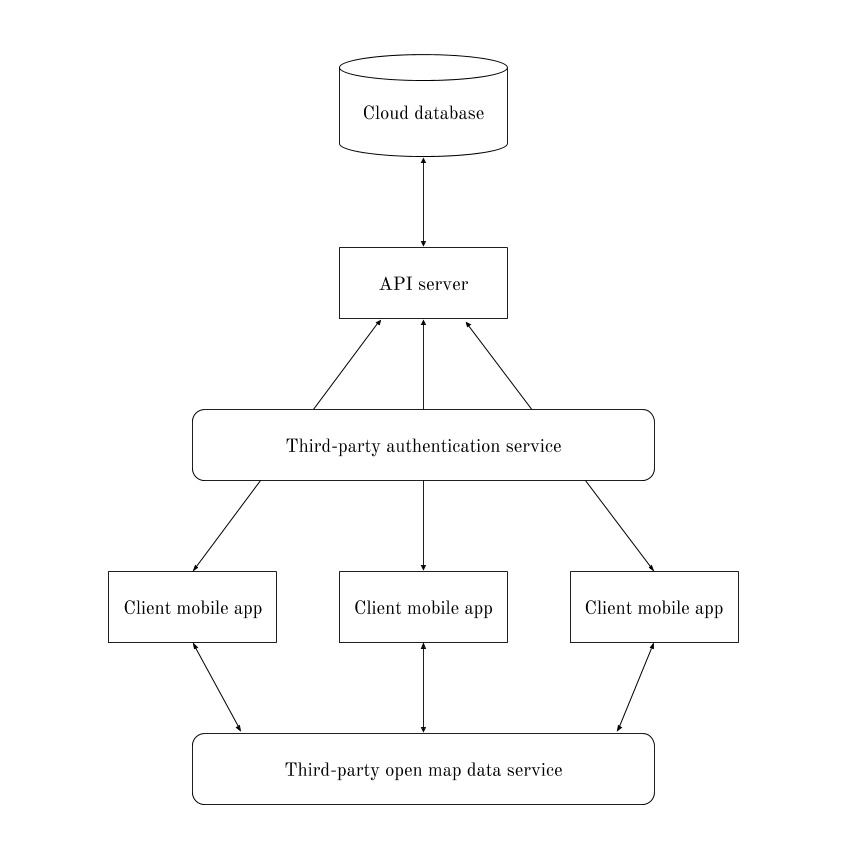
\includegraphics[scale=0.5]{images/overall_architecture.png}
  \caption{Overall architecture of the prototype}
  \label{fig:overall_architecture}
\end{figure}

All centralized data was stored in one mLab cloud-hosted MongoDB database. The database was comprised of three collections: \textit{users}, \textit{reviews}, and \textit{datapoints}. Since MongoDB is a noSQL database technology, the database schema was not actually determined on mLab, but rather within the logic of the back-end server, which is discussed in detail in section~\ref{sec:backend_architecture}. In addition to a web-based user interface, mLab provides a built-in API for accessing and modifying their hosted databases. We used the user interface for moderation purposes but the main database connection made use of the API.

The back-end server was the only component that directly interfaced with the database. It served the purpose of controlling data lookups and update requests from the user-facing clients, thereby connecting all the users of the app with each other.

The user-facing client interfaced with the back-end server through a second, custom-built API with whitelisted actions and parameters. Access to this API was federated through a third-party authentication service, provided by Auth0. Implementing authentication directly within the back-end server could have improved stability and efficiency, but we chose the external authentication service in order to reduce development time and limit the risk of security bugs.

The front-end mobile app interfaced with the authentication system by redirecting the user to the Auth0 sign-in page in an in-app browser window. After a successful sign-in attempt, the sign-in page would redirect back to the app, returning a time-limited authentication token. This token could be verified via the Auth0 API whenever a request for user data was initiated.

The mobile app also interfaced with one final service, the OpenStreetMap public API, in order to acquire high-quality basemap tiles for the in-app map. Requests to this interface were handled entirely by the Leaflet.js package, which loads OpenStreetMap basemap data by default.

One advantage of this service-based approach is that each of the five components could be swapped out for another design solution, with only minor reconfiguration of the other components. For example, future implementations could switch to a different database, authentication, or basemap service if the third-party services we selected were not desired. The user-facing client app could easily take other forms too, for example as a browser-based web app.


\section{Back-End Sever Application}
\label{sec:backend_architecture}

We implemented the back-end server as a typical lightweight Node.js application. This made for easy deployment to Heroku, the free service we chose for hosting, and tight integration with both the MongoDB database and the React front-end via the Express.js package. This combination of MongoDB, Express, React and Node is popular for its flexibility and commonly referred to as the MERN stack.

The server application is made up of five core files, three of which define the database schema. The entire codebase can be found on GitHub.\footnote{https://github.com/lbraun/geofreebie-backend}

The main file, \textit{server.js}, contains the core logic of the server including the database connection and API routes. The database connection is handled by Mongoose, an open source node package that provides object-document mapping for MongoDB. The server listener and routing are handled by Express.

The \textit{package.json} file defines these and other dependencies of the application. In addition to Mongoose and Express, we used Body-Parser to parse the HTML requests, and Cors to handle cross-origin requests. The package file also defines other configurations, like the name, version, and license of the app.

The three remaining files specify the database schema and associated models, i.e., how Mongoose should map the database documents into JSON objects and back again. The model defined in the \textit{user.js} file represents one user of the mobile app. This model includes demographic information on the user, user-specific settings, and information about what the user is offering (if anything). In future implementations, we plan to extract offers to their own model, which would allow for more than one offer per user, the saving of old offers, and other functionality that did not make it into the first prototype.

The \textit{review.js} file defines a model representing user feedback on the delivery of an offer to another user. Thus, each review object is linked to two users. The other fields of the review object model contain the users' responses to the questions about the interaction, the date of the review, and information about the offer that was exchanged. This enabled us to perform active experience sampling during the prototype evaluation, as described in section~\ref{sec:active_sampling}. We also plan to use these reviews to support the development of user trust and reputation in future implementations, by allowing users to browse public reviews before deciding to meet another user.

The \textit{datapoint.js} file defines a model that solely exists to enable this research project and not to provide any functionality to the user. Each time a user updates something in the system, a datapoint is logged with information about what the user changed. This enabled us to perform passive experience sampling during the prototype evaluation, as described in section~\ref{sec:passive_sampling}.

The server exposes eight API routes related to the first two models: five for the user model and three for the review model (see table~\ref{tab:api_routes}).

% requires \usepackage[table,xcdraw]{xcolor}
\begin{table}[ht]
\centering
\begin{tabular}{|l|l|l|}
\hline
\rowcolor{lightgray}
{\color[HTML]{333333} \textbf{Method}} & {\color[HTML]{333333} \textbf{Route}} & {\color[HTML]{333333} \textbf{Description}}  \\ \hline
GET                                    & /users                                & Find all users                                     \\ \hline
POST                                   & /users                                & Find or create a new user \\ \hline
GET                                    & /offer\_pictures/:user\_id            & Find an offer photo by user id                     \\ \hline
GET                                    & /users/:user\_id                      & Find a user by id                                  \\ \hline
PUT                                    & /users/:user\_id                      & Update a user by id                                \\ \hline
GET                                    & /pendingReviews                       & Create a new review for a given user               \\ \hline
POST                                   & /pendingReviews                       & Find reviews by user                               \\ \hline
PUT                                    & /pendingReviews/:review\_id           & Update a review by id                              \\ \hline
\end{tabular}
\caption{Prototype back-end API route}
\label{tab:api_routes}
\end{table}

\subsubsection*{Image Storage and Transmission}

One key design consideration was how to store and transmit images. According to our needs assessment, images are essential for freecycling because they are often the best way to describe what is being offered. However, images often require separate storage infrastructure, take up a lot of storage resources, and may deplete a user's mobile data quota when loaded on their mobile phone.

We decided to store images as base64 encoded strings. Base64 encoding turns binary image data into ASCII text and is one built-in destination type option of the Cordova camera plugin that we used. The benefit of this format is that it can be stored and transmitted just like all other ASCII text data. In the context of the prototype, this means that an update to an offer's picture works the same way as an update to the offer's title, and both are stored as the same kind of simple string attribute on the offer object in the application's database.

One common downside to this approach is that handling these ``data URLs'' can be very memory intensive on a mobile phone and can cause app crashes and errors. This was not a concern for us because users only need to take one photo at a time. Through early testing on an old phone with limited memory, we discovered one photo was not enough to cause problems, even when using a high image quality setting. We additionally reduced the quality of all images to 25 percent of the original quality in order to reduce data use.

A second reason mobile and web developers avoid base64 encoded images is that they are not treated the same way as standard binary-encoded images when loaded by most browsers (including the WebView of Cordova apps). Standard images are loaded last, such that the user does not have to wait for heavy images to load completely before seeing other lighter content. Images will also display partially as they are loaded, slowly growing to their full size.

We implemented a solution that provides these benefits and keeps API payloads small while still using base64 encoding for image uploads and storage. Instead of sending offer photos along with the rest of the offer information, the server sends a URL for another API request to the offer pictures endpoint. This endpoint takes the base64 encoded images from the database and converts them on the fly to serve them as standard PNG encoded images. This delays the downloading of image data until the user really needs it, and allows pictures of offers to load like any other image would.


\section{Front-End Mobile Application}
\label{sec:frontend_architecture}

The structure of the front-end mobile app was defined by Cordova application architecture conventions. Cordova applications have a web application at their core, which is supplemented by Cordova plugins and integrated into the mobile operating system via a special HTML rendering engine called WebView (see figure~\ref{fig:cordova_architecture}).

\begin{figure}[ht]
  \centering
  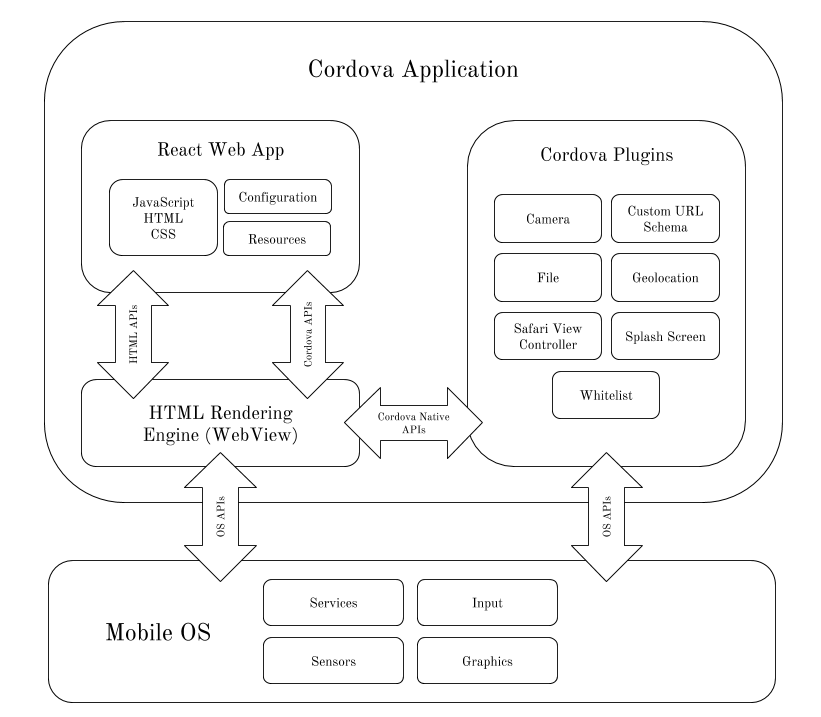
\includegraphics[scale=0.5]{images/cordova_architecture.png}
  \caption{Cordova application architecture}
  \label{fig:cordova_architecture}
\end{figure}

In this case, the core web application is built with React, so the architecture is also influenced by React conventions. We also added one directory to house the source files for a static documentation website. The complete source code for the Cordova application and the documentation website can be found on GitHub.\footnote{\url{https://github.com/lbraun/geofreebie}} In the following three subsections, we describe the web app, the plugin ecosystem, and the documentation website architecture in greater detail.

\subsubsection*{React application structure}

The files for the React app are primarily contained in four directories: \textit{node\_modules}, \textit{res}, \textit{src}, and \textit{www}. Additionally, two configuration files define how the app is packaged for distribution. The first, \textit{config.xml}, is a platform-agnostic global configuration file that contains settings for the entire Cordova app. The second, \textit{package.json}, is a standard JavaScript configuration file that controls many aspects of the React app's behavior.

The \textit{node\_modules} directory contains all the dependencies of the React app. These dependencies are defined in the \textit{package.json} configuration file.

The \textit{res} directory contains the visual resources required by the Cordova app configuration, such as the application icon and the splash screen graphic at different resolutions for different operating systems. The number and nature of these files is defined in the \textit{config.xml} configuration file.

The \textit{src} directory contains the bulk of the source code for the React application. It is divided into three sub-directories: one for business logic components, one for static data components, and one for user interface components. Figure~\ref{fig:ui_architecture} provides an overview of all the UI components and their hierarchy.

\begin{figure}[ht]
  \centering
  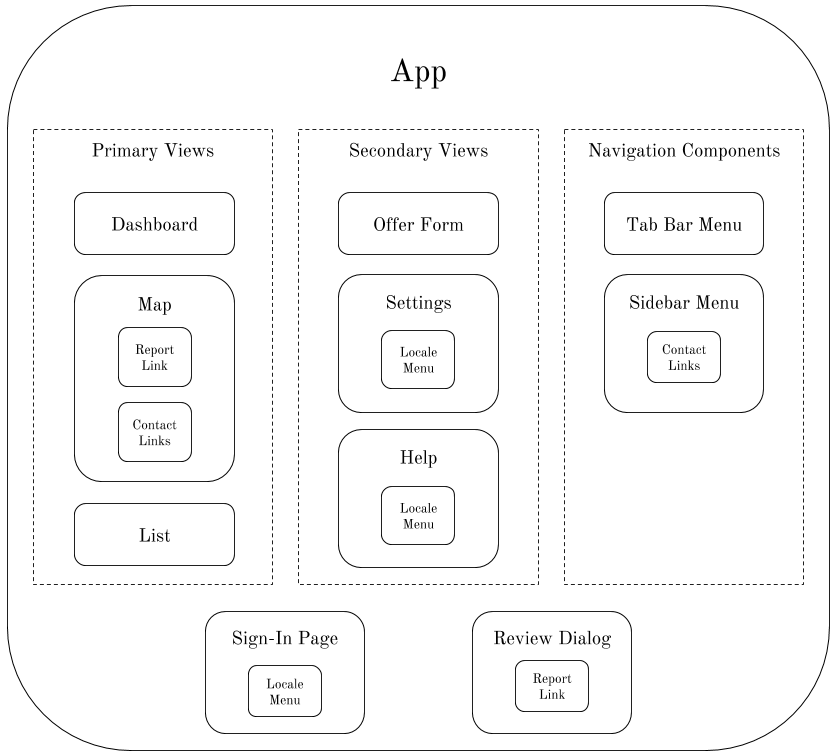
\includegraphics[width=\textwidth]{images/ui_architecture.png}
  \caption{UI components of the app}
  \label{fig:ui_architecture}
\end{figure}

The \textit{www} directory contains static web files such as images and the \textit{index.html} file, the container for all the dynamic content. It also contains the \textit{lib} directory, where the Leaflet and Onsen UI source code are housed.

\subsubsection*{Cordova plugins}

The prototype makes use of seven different Cordova plugins, which are contained in the \textit{plugins} directory:

\begin{itemize}
  \item The \textit{Custom URL Schema} plugin allows the app to be started by calling it with a URL. This is necessary for redirecting back to the app after authenticating with Auth0.
  \item The \textit{Camera} plugin provides an API for taking photos with the system's camera.
  \item The \textit{Geolocation} plugin provides information about the device's location as available based on the device's positioning hardware and software.
  \item The \textit{File} plugin allows the app to access files on the device via an API. This is used for logging in the LBS-Engine.
  \item The \textit{Safari View Controller} plugin allows the app to make use of browser technologies on iOS and Android platforms that are faster than the built-in WebView, and is the recommended way to launch a browser in Cordova apps.
  \item The \textit{Splash Screen} plugin displays and hides a splash screen during application launch.
  \item The \textit{Whitelist} plugin controls which URLs are accessible via the in-app browser.
\end{itemize}



\subsubsection*{Documentation website architecture}

The GitHub repository additionally contains the source files for a static documentation website,\footnote{\url{https://lbraun.github.io/geofreebie/}} served automatically by the GitHub Pages service.
The files for the documentation website are all contained in the \textit{docs} directory, as per GitHub Pages convention.

The documentation website is made up of four simple HTML web pages and two PDFs. The landing page, \textit{index.html}, gives an overview of the site and provides links to the other resources. \textit{contact.html} provides information about how to contact the app creator. \textit{privacy\_policy\_de.html} and \textit{privacy\_policy\_en.html} contain the privacy policy in German and English, respectively. The two PDFs, \textit{consent\_form\_de.pdf} and \textit{consent\_form\_en.pdf}, are the study consent form in German and English, respectively.
